\documentclass[tog]{acmsiggraph}
\usepackage{color}
\usepackage{overpic}
\usepackage{amssymb}
\usepackage{graphicx}
\usepackage{epstopdf}
\usepackage{amsmath}
\usepackage{graphicx}
\usepackage{amsfonts}
\usepackage{enumitem}
\usepackage{multirow}
\usepackage{algpseudocode}
\usepackage{algorithm,algorithmicx}
\usepackage[dvipsnames]{xcolor}


% \usepackage{cite}


%% 
%% Insert symbols on figures
%%
\usepackage{overpic}
\usepackage{currfile} % \currfiledir
\usepackage{wrapfig}
\usepackage{graphicx}
\usepackage{caption} % \caption*

%% 
%% More compact paragraphs
%%
\renewcommand{\paragraph}[1]{\textbf{#1}}

%% 
%% Bibliography
%% 
% \usepackage[backend=biber,sorting=ydnt,style=alphabetic,citestyle=alphabetic,maxbibnames=99]{biblatex}

%%
%% text layout
%%
% Insert whitespace at the end of a paragraph
\setlength{\parskip}{.5\baselineskip}%
% Don't intent by default on new paragraph
\setlength{\parindent}{0pt}%

%% 
%% To define colors
%% 
\usepackage{color}
\definecolor{lightgray}{rgb}{0.64, 0.64, 0.64}
\definecolor{mygray}{gray}{0.6}

%% 
%% Portions that {need major work, comments}
%% 
\newenvironment{draft}{\color{red}}{\color{black}}
\newcommand{\INSTRUCTIONS}[1]{{\textcolor{blue}{[INSTRUCTIONS] #1}}}
% \newcommand{\copypaste}[1]{{\textcolor{blue}{#1}}}
\newcommand{\copypaste}[1]{{{#1}}}
\newcommand{\OK}{{\textcolor{green}{OK!}}}
\newcommand{\todo}[1]{{\textcolor{red}{#1}}}
\newcommand{\TODO}[1]{{\textcolor{red}{[TODO: #1]}}}
\newcommand{\ignore}[1]{}

%% 
%% Inlined comments
%% 
\newcommand{\AT}[1]{{\textcolor{blue}{[AT: #1]}}}
\newcommand{\Anastasia}[1]{{\textcolor{PineGreen}{[Anastasia: #1]}}}

%% 
%% Performs the following type of transformation:
%%   \Fig{figname} => Fig.~\ref{fig:figname}
\newcommand{\Fig}[1]{Fig.~\ref{fig:#1}}
\newcommand{\Figure}[1]{Figure~\ref{fig:#1}}
\newcommand{\Eq}[1]{Eq.~\ref{eq:#1}}
\newcommand{\Sec}[1]{Sec.~\ref{sec:#1}}
\newcommand{\Section}[1]{Section~\ref{sec:#1}}
\newcommand{\Appendix}[1]{Appendix~\ref{app:#1}}
\title{Convolution surfaces model  for hand tracking}
\author{}
\pdfauthor{Secret}

\teaser{
    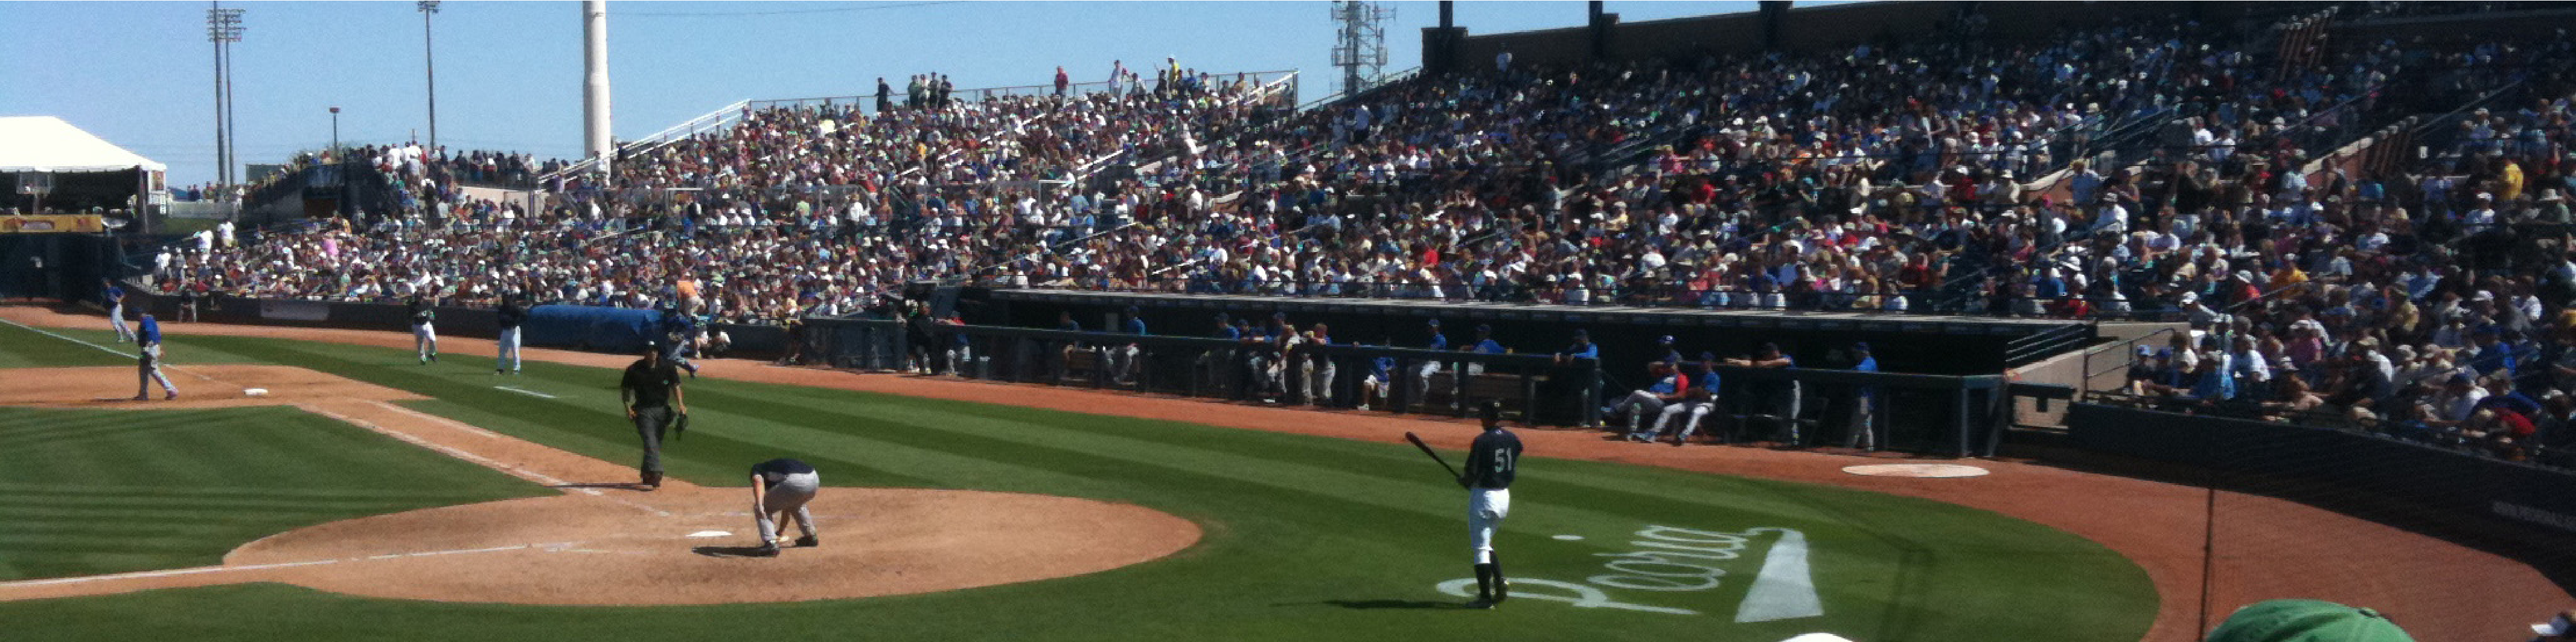
\includegraphics[height=1.5in]{fig/sampleteaser.pdf}
    \caption{Spring Training 2009, Peoria, AZ.}
}

\begin{document}
\maketitle

% !TEX root = ../hmodel.tex

\begin{abstract}
%--- Background
Modern systems for real-time hand tracking rely on a combination of discriminative and generative approaches to robustly recover hand poses. Generative approaches require the specification of a geometric model.
%--- Core point
In this paper, \todo{we propose a the use of sphere-meshes }as a novel geometric representation for real-time generative hand tracking. 
% 
\todo{How tightly this model fits a specific user heavily affects tracking precision.}
%--- Model Adaptation
We derive an optimization to non-rigidly deform a template model to fit the user data in a number of poses.
% \Anastasia{Initial transformations of the fingers are as important for tracking as precise geometry. We find both geometry and transformations.}
% \AT{this is already captured by ``dynamic geometry''?}
% 
% 
%--- Performance
This optimization jointly captures the user's static and dynamic hand geometry, thus facilitating high-precision registration.
At the same time, the limited number of primitives in the \todo{tracking template} allows us to retain excellent \todo{computational} performance. We confirm this by embedding our models in an open source real-time registration algorithm to obtain a tracker steadily running at 60Hz.
%
%While the convolution model fits the model tightly, allowing high-precision registration, the limited number of primitives in the model allows us to retain excellent tracking performance. We confirm this by embedding our models in an open source real-time tracking algorithm and obtaining a tracker steadily running at 60 frames per second.
% \Anastasia{Moreover, we introduce the fist model type that represents all the degrees of freedom of a real hand without introducing non-existing degrees of freedom. The model type allows to natively specify whether the current part is rigid, articulated or elastic.}
% \AT{It might be risky to say this... People might say: you can just use dimensionality reduction}
% \Anastasia{The increased tracking fidelity of the model has allowed us NOT TO USE RE-INITIALIZATION AT ALL. The absence of re-initialization component in our system is not a drawback of our approach, there is nothing that prohibits to add it. Our intension is to push pure tracking as far as possible and to demonstrate its power.}
% \AT{Yes, this is a good point, but we should say this in the introduction.}
%--- Why should I believe you?
We demonstrate the effectiveness of our solution by qualitatively and quantitatively evaluating tracking precision on a variety of complex motions. We show that the improved tracking accuracy at high frame-rate enables stable tracking of extended and complex motion sequences without the need for \todo{per-frame} re-initialization.
%
%--- Data release
To enable further research in the area of high-precision hand tracking, \todo{we publicly release source code and evaluation datasets.}
% together with the corresponding evaluation metrics.
\end{abstract}
% !TEX root = ../hmodel.tex
% Problem Statement: What's the problem you want to solve?
% 
% Motivation: Why is this an interesting problem? Who cares about it? Why now? Why is it appropriate for the conference audience?
% 
% Research Gap, Novelty: Why is new research required? Why can the problem not be solved with existing methods? How does the proposed solution differ from and/or improve upon existing work?
% 
% Technical Contribution: What's the key technical idea to solve the problem? Why is it beautiful?
% 
% Applications / Future Work: What will your solution enable? How does it project into the future? How will it inspire future work?



% NOTE: the paragraph names can be removed later on
\section{Introduction}
With the imminent advent of consumer-level virtual and augmented reality technology, the ability to interact with the digital world in the most natural way, using our hands, becomes of paramount importance. 
% 
We believe the degree of immersion in the virtual world will be directly correlated to whether one can use his hands to precisely interact with digital content. 
% 
% Most importantly, the degree of immersion in a virtual world is directly correlated to whether the user perceives his own realistic hands~\todo{\cite{immersion}}.
\AnastasiaComment{I think that most important is that tracking model exactly repeats the user motion, so that fine scale operations with virtual world can be performed. Otherwise, the user experience will be just pure frustration. The calibration is particularly crucial for the poses when fingers touch each other, because this is characteristic of precise operations with a hand}.
%
Over the past two decades the research community has explored a number of techniques to address this problem, from expensive and unwieldy marker-based mocap~\cite{mocapsurvey} to instrumented gloves~\cite{dipietro2008survey} as well as imaging systems~\cite{erol2007survey}. Multi-camera imaging systems can recover the hand pose and hand-objects interactions with high accuracy~\cite{ballan2013salient}, but the only system capable to approach interactive applications is the ~10 fps system of~\cite{sridhar2013multicam}. Conversely, in this paper we focus on hand motion tracking with a single RGBD sensor (e.g.\ Intel RealSense or Microsoft Kinect), as commonly predicted to be readily available in a typical AR/VR consumer experience.

\paragraph{Tracking: discriminative v.s. generative}
Modern systems for real-time tracking from RGBD data  \cite{sridhar2015fast,sharp2015accurate} rely on a combination of \emph{discriminative} approaches like \cite{keskin2012hand}, and \emph{generative} approaches such as \cite{oiko2011hand}. The per-frame re-initialization of discriminative methods prevents error propagation by offering a continuous recovery from tracking failure. As these discriminative models are learned from data, they typically only estimate a coarse pose. Therefore, generative models are used to refine the estimate by aligning a geometric template of the user hand to the measured point cloud and to regularize its motion through time. It is not surprising that the quality of the template directly affects the quality of pose refinement; see \Figure{teaser}. 

\begin{figure}[b!]
\centering
\begin{overpic} 
[width=\linewidth]
% [width=\linewidth,grid,tics=10]
{fig/coarsemodel/calibration}
% \put(75,10){{\Large TODO}}
\end{overpic}
\vspace{-.25in}
\caption{
% 
% 
(left) Tracking when the model from \protect\cite{tagliasacchi2015robust} is used without proper coarse scale calibration. (middle) A roughly manually calibrated model can help increasing the fitting fidelity, but tuning becomes increasingly difficult with more degrees of freedom. (right) The proposed automatically calibrated model. 
% 
% 
}
\label{fig:coarsemodel}
\end{figure}

The main goal of this paper is to explore novel tracking models that strike an optimal balance between accuracy and performance.
% 
\AnastasiaComment{I think, we can argue, that our model has both better performance and better accuracy for tracking. Probably here you implicitly mean that cylinder model has better performance and triangles model has better accuracy (maybe this should be discussed somewhere). I believe that the additional degrees of freedom of triangular mesh do not help, they actually make it worse. Both for calibration (because the prior is required and it gets really slow) and for tracking (because the fingers bend like they are made of gum, and it is not only rubber band effect, the fingers just do not feel as rigidly articulated objects (just have a look at Sharp sequences again). Triangular mesh could arguably be better for a high quality hand visualization, \textbf{but it does not mean that you have to track with it}. The underlying problem has much lower dimensionality. And the sensor data is not that good anyway, you cannot bet something like fingernails from it.} 
% 
More specifically, we propose a geometric model that more accurately captures the user's hand geometry, while retaining the ability to answer registration queries in closed form with very high efficiency. In \Figure{coarsemodel} and \todo{Video [00:00]} we illustrate the importance of employing a tracking template that strikes this delicate balance.

% \paragraph{Model calibration.}
% As generative models perform tracking by fitting a geometric model to what is measured by the sensor, our template should be able to represent well the observed data. However, even in modern trackers, the discrepancy between the optimal model pose given the data and the true hand pose can be significant. For example, the sources of discrepancy in \Figure{coarsemodel} include the incorrect length of fingers and the lack of the \todo{[pinky-ring]} degree of freedom. \todo{In the literature, the creation of user-specific models for tracking is referred to as \emph{calibration}.}


\paragraph{Implicit v.s. explicit templates}
In modern digital production representing objects by a surface mesh of their boundary (e.g.\ triangle or quad meshes) is the de-facto standard. Fast rendering and easy direct manipulation make \emph{explicit} surface representation attractive for many applications.
%
However, unlike \emph{implicit} models~\cite{bloomenthal1997book}, explicit representations cannot efficiently answer queries such as the distance from a point to the object's boundary, or whether a point lies inside/outside the model~\cite[Ch.1]{botsch2010book}. In tracking applications these queries play a fundamental role, as the optimization attempts to find configurations where the average \emph{distance} from model to data is minimized. Similarly, a tracker should prevent the model from assuming implausible configurations, for example by preventing self-intersections as measured by inside/outside predicates. For all these reasons, implicit models appear optimal for registration applications; indeed, compelling results in joint rigid registration and reconstruction~\cite{newcombe2011kinfu} as well as its recent non-rigid variant~\cite{newcombe2015dynfusion} leverage implicit models. One important observation is that such techniques assume the frame-rate is high compared to motion velocity, a condition that is in general not satisfied in our setting.  To address this challenge, we propose to employ a \emph{hybrid} model for tracking combining the advantages of explicit and implicit representations.

\begin{figure}[t!]
\begin{overpic} 
[width=\linewidth]
% [width=\linewidth,grid,tics=5]
{fig/convsurf/item.pdf}
\put(25,49){\small{$\mathcal{M}$}}
\put(74,49){\small{$\mathcal{M}$}}
\put(9,46){\small{$m_1$}}
\put(40,44.5){\small{$m_2$}}
\end{overpic}
\vspace{-.3in} 
\caption{
% 
% Thanks: ryoichi_sig13
The mesh {\small$\mathcal{M}$} explicitly identifies sphere positions and controls the union convolution operator to generate an implicit function. The zero-crossing of this implicit function describes the convex-hull of our spheres. \TODO{bug? bottom-left I cannot set the circle stroke size to zero, it becomes a dashed line}
% 
% 
}
\label{fig:convsurf}
\end{figure}

\paragraph{Hybrid tracking model}
The model we propose in this paper is a variant of a convolution surface~\cite{bloomenthal1991convolution}, and its fundamental building blocks are illustrated in \Figure{convsurf}. Such a construct is nothing but the zero iso-surface of the scalar function:
\begin{equation}
\phi(\mathbf{x}) = \min \int_{\mathbf{c} \in \skeleton} \mathcal{B}_{\mathbf{c}, r(\mathbf{c})}(\mathbf{x}) \: d\mathbf{c},
\label{eq:convsurf}
\end{equation}
where $\skeleton$ is a skeletal control mesh (a segment or a triangle in the simple examples of \Figure{convsurf}), and $\mathcal{B}$ is the implicit function of a sphere parameterized by its center $\mathbf{c}$ and radius $r$:
\begin{equation}
\mathcal{B}_{\mathbf{c}, r(\mathbf{c})}(\mathbf{x}) = \|\mathbf{x}-\mathbf{c}\|^2 - r(\mathbf{c})^2.
\end{equation}
The sphere centers $\mathbf{c}$ span the skeleton $\skeleton$, while the radii are a function of the position $\mathbf{c}$ within an element, linearly interpolated from values $r_*=r(c_*)$ specified on the skeletal mesh vertices $c_*$. This is indeed a \emph{hybrid} model, as \Eq{convsurf} defines an implicit surface $\surface = \{\mathbf{x} \in \mathbb{R}^n | \phi(\mathbf{x})=0 \}$, while the underlying skeleton $\skeleton$ is an explicit representation (i.e.\ a simplicial complex). We generalize this construct to devise a model suitable to represent a human hand; see \Figure{topology}.
While the integral in \Eq{convsurf} might appear complex to evaluate, distances to $\surface$ can conveniently be computed by querying distances to the piecewise linear elements of $\skeleton$; see \Figure{convsurf}.

\begin{figure}[h]
\centering
\begin{overpic} 
[width=\linewidth]
% [width=\linewidth,grid,tics=10]
{fig/topology/item.pdf}
%{fig/topology/topology}
% \put(10,10){\todo{fig:topology}}
\end{overpic}
\caption{(left) the underlying skeleton $\skeleton$ that parametrizes the convolution surfaces and a representation of the radii defined at each vertex, solid parts are shown in dark green, articulated parts in purple and elastic parts in light green.
 (right) the surface $\surface$ can be ray-traced in the fragment shader, triangulated or rendered as a set of capsule models \Figure{convsurf}-(right). \TODO{anastasia: only have 2x rendering -- the two in the left column to be precise. Also it would be a good idea to change the colors of segments v.s. spheres, no?} \TODO{color-code rigid parts of topology, and mention it in the caption} }
\label{fig:topology}
\end{figure}
\paragraph{Tracking and calibration with convolution models}
Our novel tracking model has two significant advantages. (1) Distance queries to $\surface$ can be executed by measuring the distance to the skeletal structure $\skeleton$. The number of elements in $\skeleton$ is significantly smaller~(30 in our model) than the number of polygons in a typical triangular mesh surface representation~\cite{thiery2013sphere}. 
Therefore, distance queries can be performed efficiently using a brute force approach, which leads to a simple algorithm that is trivially parallelizable and executes at a fixed frame-rate. (2)~The parameterization of our hand model is compact, as we can generate a family of models by simply adjusting \emph{positions} and \emph{radii} of the control skeleton vertices $c_* \in \skeleton$. This allows adapting the model to the hand geometry of a specific user.

\paragraph{Contributions}
% Technical Contribution: What's the key technical idea to solve the problem? Why is it beautiful?
% Applications / Future Work: What will your solution enable? How does it project into the future? How will it inspire future work?
%In our research we identify a number of contributions:
%
The core contribution of this paper is to demonstrate that convolutional models provide superior hand tracking performance for single-view depth  sensors.  We introduce an optimization approach that allows adapting our tracking model to different human hands with a high level of accuracy. 
%In addition, instead of relying on an artist-built IK skeleton, we automatically identify the kinematic decomposition of motion from data.
The improved geometric fidelity compared to existing representations leads to quantifiable reductions in registration error and allows accurate tracking even for intricate hand poses and complex motion sequences that previous methods have difficulties with. 
At the same time, due to a very compact model representation and closed-form correspondences queries, our generative model retains high computational performance, leading to sustained tracking at 60 FPS.


%(1)~We demonstrate that convolutional models can be effectively employed for tracking of geometry in motion. 
%(2)~Amongst many possible variants, we identify an effective convolution surface  topology for hand-tracking. \AT{won't they us to compare against other topologies?} \MP{Yes, I would probably not state it like this. We have no evidence that we provide the best topology, we just found one that works. I would take this out of the contributions.}
%(3)~We demonstrate that the increased model accuracy does not aberrate tracking performance, leading to a 60 FPS tracking algorithm.
% (3) While any geometric model could be employed in tracking applications, it is imperative to determine whether a model is suitable for real-time tracking applications; we demonstrate this is the case by integrating our models in an open-source tracking system~\cite{tagliasacchi2015robust} and retaining 60 FPS tracking performance. 
%(4)~We introduce an optimization technique for convolution models that adapts a given template to a given user, and demonstrate how this results in substantial improvements in tracking precision.
%(5)~Rather than relying on a artist-built IK skeleton, we define an optimization problem to automatically identify the kinematic decomposition of motion from data.

%
%%
%\hspace{0in}
%%
%\MP{I would not list future work in the contributions section. It somewhat limits our contribution as we are already pointing to things that we did not do.}.
%%--- Areas of future work
%Our findings pave the way to a number of interesting venues for future works, including 
%(1)~the extension of our modeling framework to the capture of generic articulated geometry in motion, 
%(2)~the consolidation of optimization for modeling and tracking stages, 
%(3)~the generation of parameterizations, so to enable texturing and level-of-detail representations for convolution models and
%(4)~\todo{the possibility to automatically discover a tracking template}. \
%% 
%% \item Proposed a single optimization framework for modeling and tracking
%% \item Skinning. Display the texture on the model. For that a  parametrization is required. Potentially create ``bumps map'' to apply the errors from model fitting stage
%% \item Automatically identifies the degrees of freedom and axes of rotation from data

\paragraph{Overview}
The remainder of the paper is structured as follows: We survey related work in \Section{related}, and describe our generative real-time tracking technique in \Section{tracking} detailing how our novel formulation enables efficient correspondence computation.
% 
\Section{modeling} explains how we build our template model from 3D scans acquired either through multi-view stereo or from depth maps.
% 
In \Section{results} we analyze the performance of our convolution surface model for realtime hand tracking and provide comparisons to alternative methods. 
% 
We conclude in \Section{discussion} with a discussion of current limitations and ideas for future work.
 

\AT{I think we should mention the videos. We have to mention something about the fact that screen-recording is very invasive and at times it interfered with framerate? (I have seen this in the video in at least two occasions)}

%%%%%%%%%%%%%%%%%%%%%%%%%%%%%%%%%%%%%%%%%%%%%%%%%%%%%%%%%%%%%%%%%%%%%%%%%
%\subsection{Contributions}

\subsubsection*{1. Suggested a hand model representation well suited for user-specific adaption, tracking and animation}

TODO: 

\begin{itemize}
\item Modeling. Implement initialization for the model fitting by running Htrack and putting the hand in a similar pose. 
\item Skinning. Display the texture on the model. For that a parametrization is required. Potentially create ``bumps map'' to apply the errors from model fitting stage. 
\end{itemize}

\subsubsection*{1a. Proposed a single optimization framework for modeling and tracking}

TODO:

\begin{itemize}
\item Run a couple of iteration of ARAP for palm after IK optimization just with data term.
\end{itemize}

\subsubsection*{1b. Developed a tracking model that represents all the degrees of freedom of human hand without creating inexistent degrees. (Not guaranteed by the other approaches, look how model adaptation paper finds the degrees of freedom)}

\subsubsection*{Improved accuracy of state-of-art hand tracking system}

TODO: 

\begin{itemize}
\item Add outline term, time interpolation of initial joint angles, downsampling of the sensor data, fingertips term.
\end{itemize}

\subsection{Contributions}

\subsubsection*{1. Suggested a hand model representation well suited for user-specific adaption, tracking and animation}

TODO: 

\begin{itemize}
\item Modeling. Implement initialization for the model fitting by running Htrack and putting the hand in a similar pose. 
\item Skinning. Display the texture on the model. For that a parametrization is required. Potentially create ``bumps map'' to apply the errors from model fitting stage. 
\end{itemize}

\subsubsection*{1a. Proposed a single optimization framework for modeling and tracking}

TODO:

\begin{itemize}
\item Run a couple of iteration of ARAP for palm after IK optimization just with data term.
\end{itemize}

\subsubsection*{1b. Developed a tracking model that represents all the degrees of freedom of human hand without creating inexistent degrees. (Not guaranteed by the other approaches, look how model adaptation paper finds the degrees of freedom)}

\subsubsection*{Improved accuracy of state-of-art hand tracking system}

TODO: 

\begin{itemize}
\item Add outline term, time interpolation of initial joint angles, downsampling of the sensor data, fingertips term.
\end{itemize}


\section{Related Literature}

\begin{itemize}

\item Albrecht et al. \cite{albrecht2003construction} developed an approach for creating an anatomically realistic hand model that includes bones and muscles structure. Their approach requires several prerequisites including plaster cast of a human hand and laser scanner for manually creating a physically realistic hand template. Given user-defined correspondences between 3D feature points and the hand image, a specific hand model is created by deforming a generic hand model. 

\item Rhee et. al. \cite{rhee2006human} use a single image of a hand at rest pose to infer joint hand joint locations from skin creases. Given the skeleton obtained at the previous step and the hand contour from the image, they deform a template hand mesh to fit this data. 

\item Straka et al. \cite{straka2012simultaneous} also fit the template mesh with attached skeleton to 3D data. The model is deformed to explain the data while keeping the vertices attached to their corresponding bones. It is on clear whether the approach whether be able to handle a hand motion sequence, since the results are demonstrated on a full body model.

\item Taylor et. al. \cite{taylor2014user} generate a user-specific hand model from an RGBD video sequence. The model is represented as a triangular mesh with an embedded skeleton. In each frame the hand pose is initialized using an appearance-based tracking algorithm. The hand model parameters are found by solving a single optimization problem formulated for the entire video sequence which also finds hand pose in each frame. 

\item Khamis et. al.  \cite{khamis12learning} fit a hand model for a specific user by finding its shape coordinates in the basis of mesh matrices and bones locations. As in the approach by Taylor et. al, they optimize simultaneously for pose and shape parameters in all the frames of an RGBD sequence across all the subjects. Requires large number of subjects as a regularization for excessive degrees of freedom. 

The results generated by the approaches listed above could be used as an input for our system to create a hand model representation adapted for efficient tracking and animation.


\end{itemize}

%\section{Tracking}

In this paper instead of a standard inverse kinematics approach for aligning the model with data we use \textit{"As Rigid As Possible"} approach~\cite{sorkine2007arap}. The hand model is parametrized with the locations of the vertices of the hand skeleton $c = {c_1, c_2, ... c_N}$.

\begin{equation}
	\min_{c} E_{ICP} + E_{ARAP} \label{eq:tracking_energy}
\end{equation}

The first energy $E_{ICP}$ models a 3D geometric registration in the spirit of ICP as

\begin{equation}
	E_{ICP} = \omega_1 \sum_{p \in P} \| p - \Pi(p, c)\|_2
\end{equation}

where $P$ is the set of data points.

The second energy $E_{ARAP}$ is needed for shape preservation. Denote locations of hand skeleton vertices at rest pose as $c^0$ and in iteration $t$ as $c^t$. Denote the set of all edges of hand skeleton as $E$.

\begin{equation}
	E_{ARAP} = \omega_2 \sum_{e \in E} \| e(c^t) - R_e e(c^0)\|_2^2,
\end{equation}

where $R_e$ is the optimal rotation to bring the rest pose edge $e^0$ to the current position $e^t$. Unless we what some set of edges to rotate as a solid body, the rotation $R_e$ can be expressed in the closed form, such that $R_e e(c^0)$ is collinear to $e(c^t)$. 
Each optimization iteration consists of two alternating steps: first we find the projections of the data points to the model surface $\Pi(p, c)$ and the optimal rotations $  R_e  $. Then we make one step of Levenberg-Marquardt iteration for energy (\ref{eq:tracking_energy}).
%% !TEX root = ../hmodel.tex
\section{Results}
\label{sec:results}


\begin{figure}[t!]
\centering
\begin{overpic} 
[width=\linewidth]
% [width=\linewidth,grid,tics=10]
{\currfiledir/item.pdf}
% \put(40,25){\todo{\Large DRAFT}}
% \put(0,-3){\todo{\currfiledir}}
\end{overpic}
\caption{
% 
Our dataset contains a number of wide range of motions that spans the entire literature on hand tracking. We identify three main axes of variations by analyzing recent hand-tracking papers, and produce a dataset that samples this space. \TODO{mention they come from teaser sequence, and position in video, 150 microseconds 9 frames}
% 
}
\label{fig:motiontypes}
\end{figure}

\todo{In our research, beyond releasing a dataset specifically designed to evaluate high precision tracking and propose metrics to quantitatively evaluate  performance in an algorithm-independent fashion.}

\subsection{Database}
\begin{DRAFT}
Lorem ipsum dolor sit amet, consectetur adipisicing elit, sed do eiusmod tempor incididunt ut labore et dolore magna aliqua. Ut enim ad minim veniam, quis nostrud exercitation ullamco laboris nisi ut aliquip ex ea commodo consequat. Duis aute irure dolor in reprehenderit in voluptate velit esse cillum dolore eu fugiat nulla pariatur. Excepteur sint occaecat cupidatat non proident, sunt in culpa qui officia deserunt mollit anim id est laborum.
\end{DRAFT}

\providecommand{\depthrend}{\mathcal{R}}
\providecommand{\metricone}{E_\text{3D}}
\providecommand{\metrictwo}{E_\text{2D}}
\subsection{Comparison Metrics}
Taylor and colleagues \shortcite{taylor2016concerto} have reported how recent hand tracking algorithms \cite{sharp2015accurate} \cite{tagliasacchi2015robust} have reached human precision in determining the location of key features (e.g. fingertips and wrist position). Therefore, publicly available datasets like \cite{tompson2014real} and \cite{sridhar2013multicam} \MP{add: ``based on human labeling'' to make it clear, but is this true for these methods?} have become less suitable for quantitatively evaluating the quality of high-precision tracking. 
% 
For this reason, we propose several easy-to-compute metrics to evaluate the quality of generative algorithms for modeling/tracking. A core element that makes these metrics appealing is that, much like key feature positions, they are completely algorithm (and hence model) independent. This is essential, as it will enable the research community to validate and compare results through quantitative analysis. 
% 
We achieve this goal by expressing these metrics exclusively as a function of the acquired depth image $\depth_n$, and of the depth image $\depthrend_{n}$ of the rendered model. Note that below we drop the subscript $n$ for notational brevity, and that $\point \in \depth$ only considers points within the RoI. \AT{We have to explain why the ``golden energy'' is not sufficient; perhaps we can say more once we see the results.}

\begin{figure}[t!]
\centering
\begin{overpic} 
[width=\linewidth]
% [width=\linewidth,grid,tics=10]
{\currfiledir/item.pdf}
% \put(0,-3){\todo{\currfiledir}}
\put(6,97){{\small $E_{3D}$ }}
\put(68.4,96.5){{\tiny \cite{tagliasacchi2015robust}}}
\put(73,94.5){{\tiny [Proposed Method]}}
\put(6,47.5){{\small $E_{2D}$ }}
\put(68.4,47.4){{\tiny \cite{tagliasacchi2015robust}}}
\put(73,45.4){{\tiny [Proposed Method]}}
\end{overpic}
\caption{
% 
%
\handyseq{teaser}
% 
% 
}
\label{fig:comp1}
\end{figure}

\paragraph{Fitting residuals (3D)}
As we are seeking high-quality alignement every pixel from the sensor data should lie in the proximity of the model. Here the $\proj_\depthrend$ computes the closest point correspondence to the point cloud of the rendered model:
\begin{equation}
\metricone = \frac{1}{|\depth|}\sum_{\point \in \depth} \| \point - \proj_\depthrend(\point) \|_2^2
\label{eq:metric1}
\end{equation}
Differently from tracking these can be fetched with a kd-tree.

\paragraph{Silhouette residuals (2D)}
Computing model-to-data registration residuals in 3D is not meaningful \todo{because blah}. Therefore, we evaluate the registration residual in the 2D projective space. 
\begin{eqnarray}
\metrictwo 
&=& \frac{1}{|\depthrend \setminus \partial\depth|} 
\sum_{\pixel \in \depthrend \setminus \partial\depth} \| \pixel - \proj_{\partial\depth}(\pixel) \|_2 \\ 
&=& \frac{1}{|\depthrend \setminus \partial\depth|} 
\sum_{\pixel \in \depthrend \setminus \partial\depth} \text{DT}(\pixel)
\label{eq:metric2}
\end{eqnarray}
Note how above each term above can be evaluated efficiently by pre-computing the 2D euclidean distance transform DT of the RoI's (image-space) silhouette $\partial \depth$. Further, note that DT evaluates to zero for a pixel inside the silhouette. 

\begin{figure}[t!]
\centering
\begin{overpic}
[width=\linewidth]
% [width=\linewidth,grid,tics=10]
{\currfiledir/item.pdf}
\put(1,30){{\small$\%$}}
\put(1,64){{\small$\%$}}
\put(93,37.5){{\small $E_{3D}$}}
\put(93,04.5){{\small $E_{2D}$}}
\end{overpic}
\caption{
% 
%
\todo{Each plot visualizes on the $y$ axis the portion of frames with a mean error metric below the value reported on the $x$ axis. We employ the \handyseq{teaser} sequence for this purpose. Curves closer to the top-left quadrant indicate better performance.}
% 
% Our method is quantitatively compared to the one of~\protect\cite{tagliasacchi2015robust} on the \handyseq{teaser} sequence.
% 
% 
}
\label{fig:comp2}
\end{figure}

\paragraph{Golden Energy}
Another metric we consider is the golden energy from Sharp and colleagues~\shortcite{sharp2015accurate} that was employed to drive their PSO real-time tracker:
\begin{equation}
E_{\text{Au}} = \sum_{ij} \rho(\depth(i,j) - \depthrend(i,j))
\label{eq:golden}
\end{equation}
where $\rho(e)=\min(|e|,\tau)$ is a truncated $\ell_1$ distance to make the metric less sensitive to outliers ($\tau=100mm$). Pixels outside the region of interest are mapped to the far plane $\depth^\text{max}$.

\begin{figure}[t!]
\centering
\begin{overpic} 
[width=\linewidth]
% [width=\linewidth,grid,tics=10]
{\currfiledir/item.pdf}
% Legend/1
\put(9,56){{\small $E_{2D}$ }}
\put(22,57.15){{\tiny \cite{tagliasacchi2015robust}}}
\put(22,55.15){{\tiny \citeme{}}}
% Legend/2
\put(44.5,56){{\small $E_{3D}$ }}
\put(57,57.15){{\tiny \cite{tagliasacchi2015robust}}}
\put(57,55.15){{\tiny \citeme{}}}
% Horizontal axis
\put(10.5,2){{\small \emph{tayl1} }}
\put(21.5,2){{\small \emph{srid1} }}
\put(32,2){{\small \emph{srid2} }}
\put(43,2){{\small \emph{srid3} }}
\put(54,2){{\small \emph{srid4} }}
\put(64.5,2){{\small \emph{shar1} }}
\put(75.5,2){{\small \emph{shar2} }}
\put(86.3,2){{\small \emph{shar2} }}
% Vertical axis
\put(4,11.3){{\small 1}}
\put(4,19){{\small 2}}
\put(4,26.5){{\small 3}}
\put(4,34.2){{\small 4}}
\put(4,42){{\small 5}}
\put(4,49.7){{\small 6}}
% 
\end{overpic}
\caption{
% 
% 
Average 2D/3D tracking performance metrics of the proposed method compared to \protect\cite{tagliasacchi2015robust}. 
% 
In the additional material we report error plots through time for the aggregated data above.
% Our calibrated convolution model often helps the generative  technique from incurring in loss-of-tracking, these are visualized are spike in the errors in the
% 
% 
}
\label{fig:barchart}
\end{figure}
\paragraph{Comparison to HTrack}
% \protect\cite{tagliasacchi2015robust}

 
\paragraph{Acknowledgements}
\begin{draft}
We would like to thank the reviewers for their feedback, Andrii Maksai, Sofien Bouaziz and Misha Kazhdan for insightful discussions, \todo{Tom Cashman, Jonathan Taylor and Andrew Fitzgibbon for their help generating the quantitative comparisons to~\cite{taylor2016concerto,sharp2015accurate}}, Chris Wojtan for his help rendering \Figure{convsurf}, Merlin Nimier-David, Pei-I Chen and Thomas Joveniaux for their help in creating calibration datasets, Matthew Murray, Laura Grondhal, Nicolas Guillemot for their help proofreading the paper. 
% 
This research is supported by the NSERC Discovery grant \#2016-05786 and the Swiss NSF grant \#200021-153567.
\end{draft}
\bibliographystyle{acmsiggraph}
\nocite{*} %<< prints out everything
\bibliography{hmodel}

\appendix
\section{Modeling}

%%%%%%%%%%%%%%%%%%%%%%%%%%%%%%%%%%%%%%%%%%%%%%%%%%%%%%%%%%%%%%%%%%%%%%%%

\subsection{Convolution segment}

\begin{figure}[h!] 
	\centering
	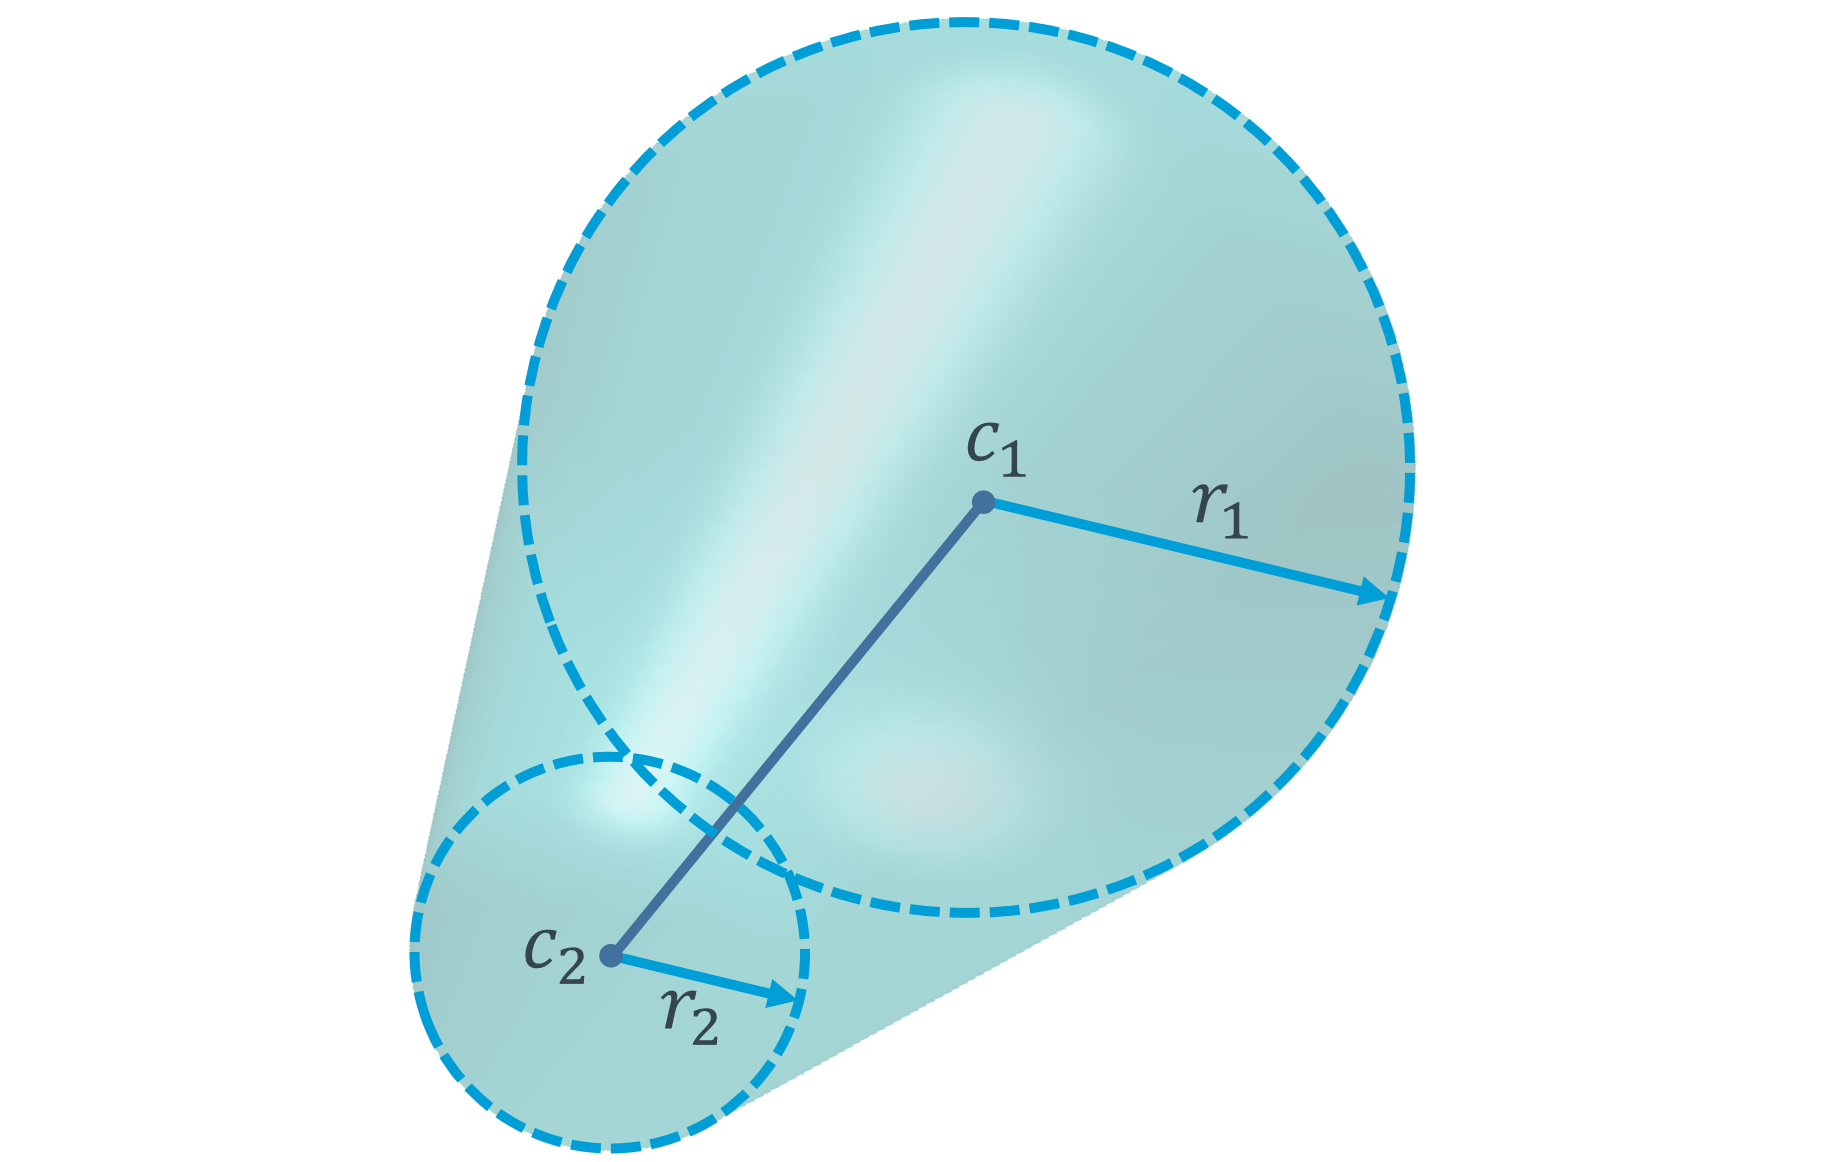
\includegraphics[width=0.5\textwidth]{fig/convsegment.png}
	\caption{Convolution segment.}
	\label{fig:convsegment}
\end{figure}

A convolution segment (Figure \ref{fig:convsegment}) is defined by two spheres $S_1 = \{c_1, r_1\}$ and $S_2 = \{c_2, r_2\}$.
Given the data points $P = \{p_i\}_{i = 1}^N$ and their projections on the model  $Q = \{q_i(c_1, c_2, r_1, r_2)\}_{i = 1}^N$  we construct a vector-function $\textbf{f}$ 

 \begin{equation}
 	\textbf{f} = \left[
 		\begin{array}{c}
 			\vdots \\
			p_i^x - q_i^x\\
			p_i^y - q_i^y\\
			p_i^z - q_i^z\\
			\vdots \\
	\end{array}
 	\right].
 \end{equation} 

\begin{figure}[h!] 
	\centering
	\hspace{-2em}
	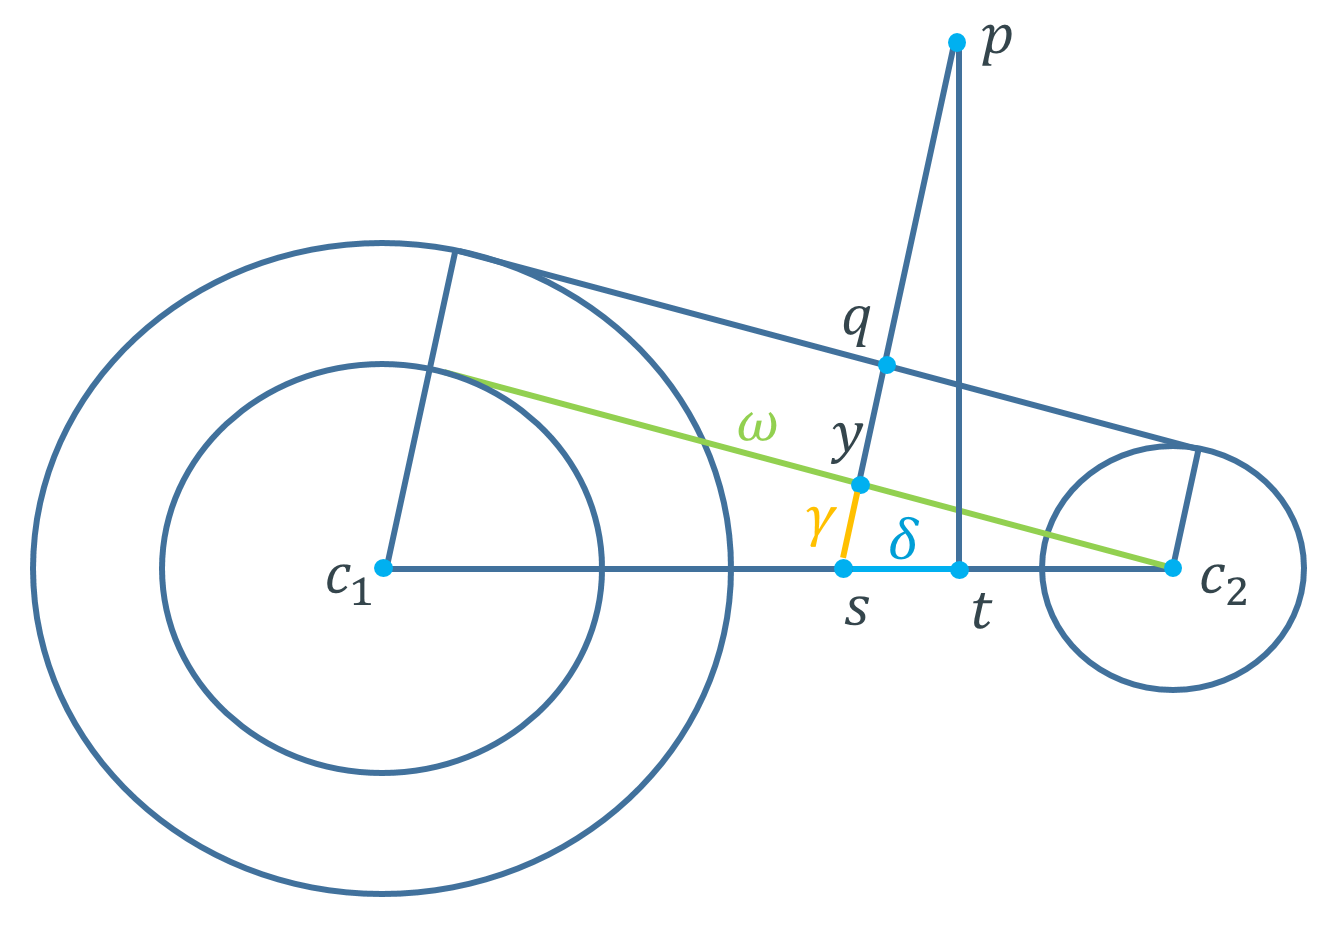
\includegraphics[width=0.47\textwidth]{fig/projection_convsegment.png}
	\caption{Convolution segment.}
	\label{fig:projection_convsegment}
\end{figure}

To fit the model to the data, we iteratively minimize $\textbf{f}$ using Levenberg-Marquardt iteration. In order to compute the Jacobian, the projections $q_i$ should be expressed as functions of model parameters. Let us first find the projection $q$ of a point $p$ on the segment $\{c_1, c_2\}$. Assume that $c_1 > c_2$. If the point on the segment $t$ closest to $p$ lies at the end of the segment, say, $c_1$, than $q = c_1 + \frac{r_1  (p - c_1)}{\Vert p - c_1 \Vert}$. 
Otherwise, the projection $q$ is computed as 

\begin{align*}
& u = c_2 - c_1, \\
& v = p - c_1, \\
& \omega = \sqrt{u^T u - (r_1 - r_2)^2}, \\
&  \delta =  \frac{(r_1 - r_2) \Vert p - t \Vert}{\omega}, \\
&   s = t - \delta  \frac{c_2 - c_1} {\Vert c_2 - c_1 \Vert}, \\
&  \gamma = \frac{(r_1 - r_2)   {\Vert c_2 - t + \delta  \frac{u} {\Vert u \Vert}} \Vert} {\Vert u \Vert}, \\
&   q = s +\frac{ (p - s) (\gamma + r_2) }{ \Vert p - s \Vert } .
\end{align*}

(See Figure \ref{fig:projection_convsegment}).

Given the projection $q_i = q_i(c_1, c_2, r_1, r_2)$, the objective function $\textbf{f} = [\cdots, f_i^T, \cdots]^T$  has the Jacobian $\textbf{J}$ with $J_{ij} = \frac{\partial{f_i}}{\partial{x_j}}$, where $\textbf{x} = [c_1, c_2, r_1, r_2]$.  At each iteration of Levenberg-Marquardt , we first compute the data-model correspondences. In case of convolution segments this amounts to determining whether the closest point is located at one of the end points of the segment or lies in between. Given this correspondence, the Jacobian is computed using chain rule, by composition of derivatives of algebraic operations required to find $q(c_1, c_2, r_1, r_2)$.


%%%%%%%%%%%%%%%%%%%%%%%%%%%%%%%%%%%%%%%%%%%%%%%%%%%%%%%%%%%%%%%%%%%%%%%%


\subsection{Convolution triangle}


\begin{figure}[h!] 
	\centering
	\hspace{-2em}
	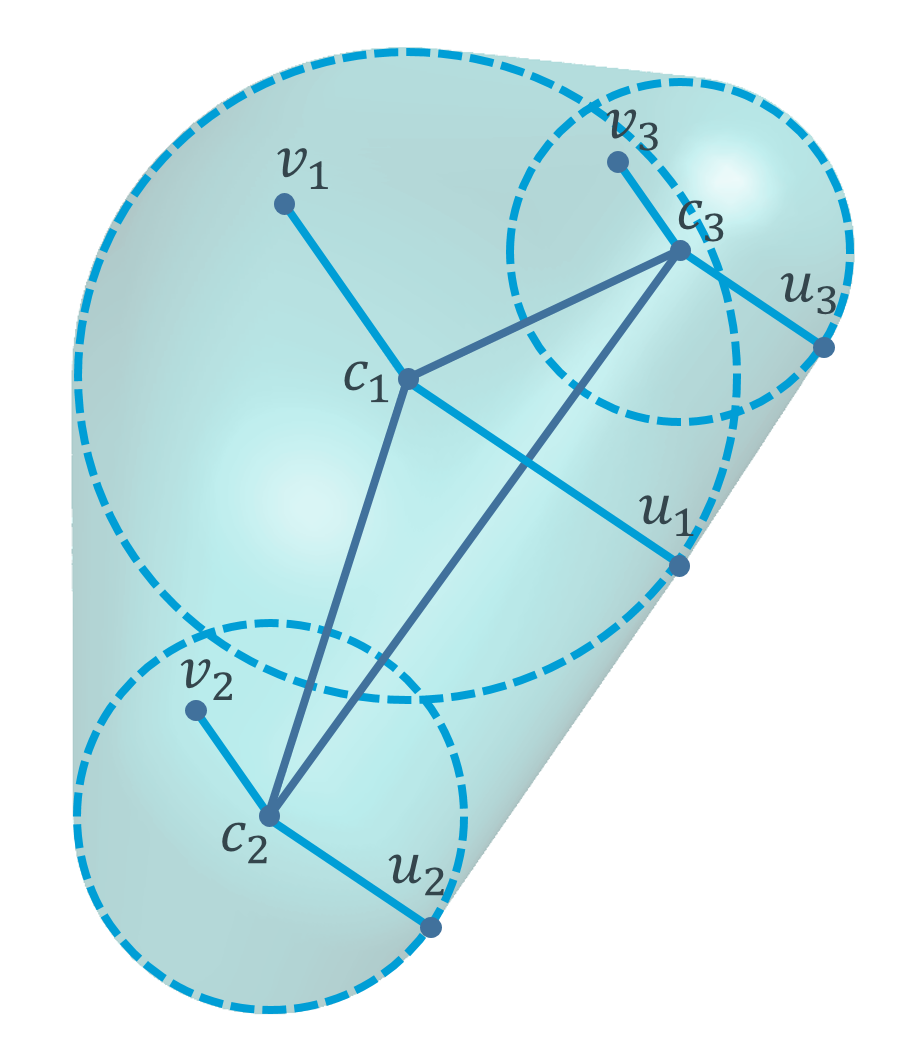
\includegraphics[width=0.3\textwidth]{fig/convtriangle.png}
	\caption{Convolution triangle.}
	\label{fig:convtriangle}
\end{figure}

A convolution triangle (Figure \ref{fig:convtriangle}) is defined by three spheres $S_1 = \{c_1, r_1\}$, $S_2 = \{c_2, r_2\}$ and $S_3 = \{c_3, r_3\}$. To express the projection $q_i$ as a function of the model parameters, first, let us find the outer tangent planes for the spheres. There exists two outer tangent planes if none of the spheres lies entirely inside of the cone tangent to the other two spheres. 

\begin{figure}[h!] 
	\centering
	\hspace{-2em}
	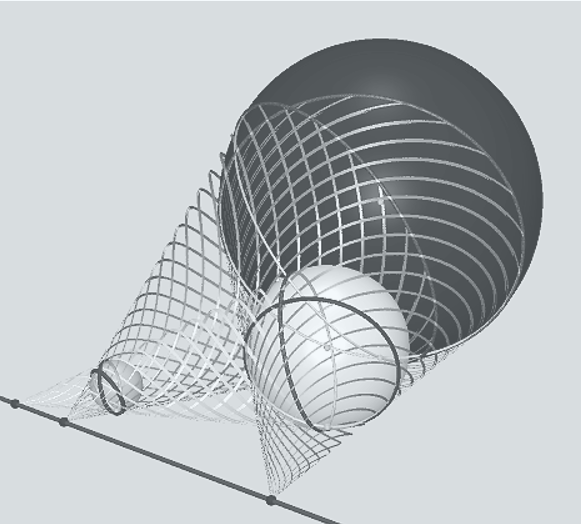
\includegraphics[width=0.45\textwidth]{fig/cones_and_tangent_plane.png}
	\caption{The three apices of the cones tangent to each pair of spheres lie on a straight line.}
	\label{fig:logistic_regression}
\end{figure}

\begin{figure}[h!] 
	\centering
	\hspace{-2em}
	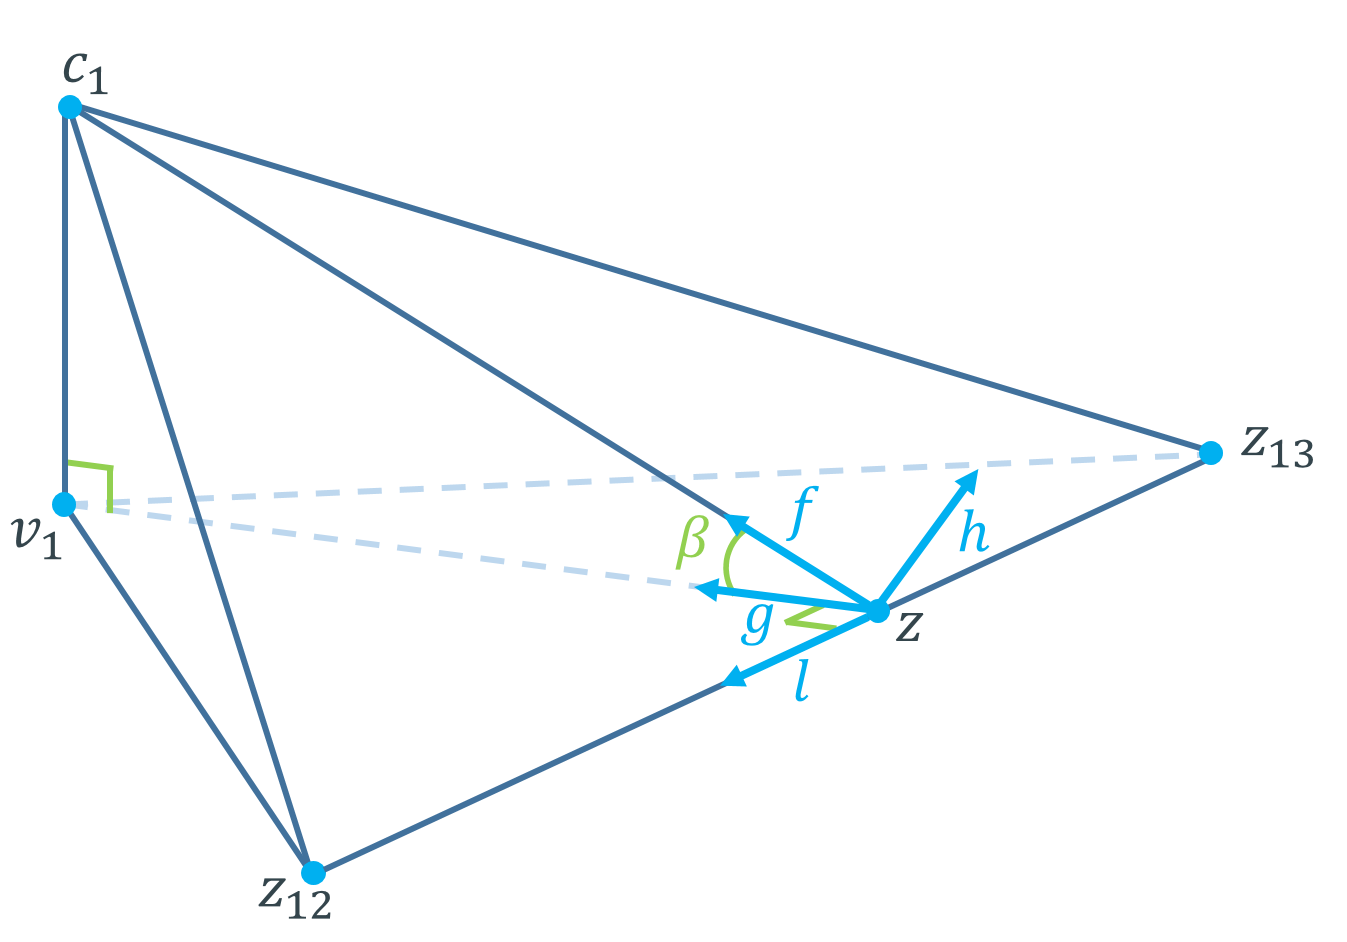
\includegraphics[width=0.45\textwidth]{fig/projection_convtriangle.png}
	\caption{Computing the tangent plane for three spheres.}
	\label{fig:projection_convtriangle}
\end{figure}

\subsection{Computing the tangent plane}

In Figure \ref{fig:projection_convtriangle}, the point $z_{12}$ is an apex of a cone tangent to the spheres $S_1$ and $S_2$. The position of $z_{12}$ can be found from similarity of triangles:

\begin{equation}
	z_{12} = c_1 +\frac{r_1 (c_2 - c_1)}{r_1 - r_2},
\end{equation}

In the same way,

\begin{equation}
	z_{13} = c_1 +\frac{r_1 (c_3 - c_1)}{r_1 - r_3}.
\end{equation}

The direction vector $l$ of the line, that contains the apices of the tangent cones is found as

\begin{equation}
	l = \frac{z_{12} - z_{13}} {\Vert z_{12} - z_{13} \Vert} 
\end{equation}

The intersection point of the plane orthogonal to $l$ and going through the point $c_1$ with the line going through $z_{12}$ and $z_{13}$ is found as

\begin{equation}
z = z_{12} + ((c_1 - z_{12})^T l )l.
\end{equation}

The sine and cosine of the angle $\beta$ in triangle $\{c_1, z, v_1\}$ are given by 

\begin{equation}
	\sin(\beta) = \frac{r_1}{\eta},
\end{equation}

\begin{equation}
	\cos(\beta) = \frac{\nu}{\eta},
\end{equation}

where $\eta = \Vert c_1 - z \Vert $ and $\nu = \sqrt{\eta^2 -  r_1^2}$. 

Denote the tangent point of the sphere $S_1$ as $v_1$. The direction vector $g$ of the line $\{c_1, v_1\}$ can be found by rotating the direction vector $f$ of the line 
$\{c_1, z\}$ by angle $\beta$ around the axis $l$.

\begin{align}
	& h = \frac{l \times f}{\Vert l \times f \Vert}, \\
	& g = \sin(\beta) h + \cos(\beta) f.	
\end{align}

The tangent point $v_1$ is found as
\begin{equation}
v_1 = z + \nu  g
\end{equation}


Having the normal vector of the tangent plane $n = \frac{v_1 - c_1}{\Vert v_1 - c_1 \Vert}$, we can find the tangent points of the spheres $S_2$ and $S_3$:

\begin{align}
	& v_2 = c_2  + r_2 n \\
	& v_3 = c_3 + r_3 n 
\end{align}

The second tangent plane $\{u_1, u_2, u_3$\} is found by rotating the vector $f$ around the axis $l$ by an angle $-\beta$.



\subsection{Computing the projection}

If the point, closest to $p$ on triangle $\{v_1, v_2, v_3\}$ or on triangle $\{u_1, u_2, u_3\}$ lies inside of the triangle, than it is the projection $q$. Otherwise $q$ belongs to the surface of one of the convolution segments $\{c_1, c_2\}$,  $\{c_1, c_3\}$, or  $\{c_1, c_3\}$. Thus, the candidates for $q$ are the projections of $p$ on the segments $q_{12}$, $q_{13}$ or $q_{23}$. The projection $q$ is determined taking into account the distance to $p$ and whether  $q_{12}$, $q_{13}$ and $q_{23}$ are located inside or outside of the segments $\{c_1, c_2\}$,  $\{c_1, c_3\}$, and  $\{c_1, c_3\}$.  

%%%%%%%%%%%%%%%%%%%%%%%%%%%%%%%%%%%%%%%%%%%%%%%%%%%%%%%%%%%%%%%%%%%%%%%%

\subsection{Combining several blocks}

Consider the case when several convolution segments and triangles are used to create a more complex model. To find the projection $q$, we compute a projection $q_j$ on each  building block.  The projection $q$ is determined taking into account the distances between $q_j$ and $p$ and whether  $q_j$ are located inside or outside of the building blocks.

%%%%%%%%%%%%%%%%%%%%%%%%%%%%%%%%%%%%%%%%%%%%%%%%%%%%%%%%%%%%%%%%%%%%%%%%


\end{document}
